\documentclass[10pt]{beamer}
\usetheme[
%%% option passed to the outer theme
%    progressstyle=fixedCircCnt,   % fixedCircCnt, movingCircCnt (moving is deault)
  ]{Berlin}
  
% If you want to change the colors of the various elements in the theme, edit and uncomment the following lines

% Change the bar colors:
%\setbeamercolor{Feather}{fg=red!20,bg=red}

% Change the color of the structural elements:
%\setbeamercolor{structure}{fg=red}

% Change the frame title text color:
%\setbeamercolor{frametitle}{fg=blue}

% Change the normal text color background:
%\setbeamercolor{normal text}{fg=black,bg=gray!10}

%-------------------------------------------------------
% INCLUDE PACKAGES
%-------------------------------------------------------

\usepackage[utf8]{inputenc}
\usepackage[english]{babel}
\usepackage[T1]{fontenc}
\usepackage{amsmath}
\usepackage{helvet}
\usepackage{multirow}
\usepackage{graphicx}
\usepackage{comment}
\usepackage[absolute,overlay]{textpos}
\usepackage{tikz}
\usepackage{amssymb}
\usepackage{textpos}
\usetikzlibrary{arrows,automata,positioning}
\usetikzlibrary{shapes.multipart}
\usetikzlibrary{decorations.markings}

\newcommand\hcancel[2][black]{\setbox0=\hbox{$#2$}%
\rlap{\raisebox{.45\ht0}{\textcolor{#1}{\rule{\wd0}{1pt}}}}#2}

%-------------------------------------------------------
% DEFFINING AND REDEFINING COMMANDS
%-------------------------------------------------------

% colored hyperlinks
%\renewcommand*{\Footnotemark}[1]{\NCC@makefnmark{#1}}
\newcommand{\chref}[2]{
  \href{#1}{{\usebeamercolor[bg]{Feather}#2}}
}
\newcommand{\tuple}[1]{{\langle #1 \rangle}}
\newcommand{\pre}{\mathsf{pre}}     % precondition
\newcommand{\eff}{\mathsf{eff}}     % effect
\newcommand{\cond}{\mathsf{cond}}   % conditional effect

\newcommand{\X}{\mathcal{X}}
\newcommand{\F}{\mathcal{F}}
\newcommand{\A}{\mathcal{A}}
\newcommand{\N}{\mathcal{N}}
\newcommand{\I}{\mathcal{I}}
\newcommand{\real}{\mathbb{R}}
\newcommand{\Dw}{\mathcal{D}}
\newcommand{\Xw}{\mathcal{X}}
\newcommand{\Aw}{\mathcal{A}}
\newcommand{\Rw}{\mathcal{R}}
\newcommand{\OO}{\mathcal{O}}
\newcommand{\tOO}{\wt{\OO}}
\newcommand{\II}[1]{\mathbb{I}{\left\{#1\right\}}}
\newcommand{\PP}[1]{\mathbb{P}\left[#1\right]}
\newcommand{\EE}[1]{\mathbb{E}\left[#1\right]}
\newcommand{\EEs}[2]{\mathbb{E}_{#2}\left[#1\right]}
\newcommand{\PPt}[1]{\mathbb{P}_t\left[#1\right]}
\newcommand{\EEt}[1]{\mathbb{E}_t\left[#1\right]}
\newcommand{\PPi}[1]{\mathbb{P}_i\left[#1\right]}
\newcommand{\EEi}[1]{\mathbb{E}_i\left[#1\right]}
\newcommand{\EEp}[1]{\mathbb{E}_{\pi,P}\left[#1\right]}
\newcommand{\EEcp}[2]{\mathbb{E}_{\pi,P}\left[\left.#1\right|#2\right]}
\newcommand{\PPc}[2]{\mathbb{P}\left[#1\left|#2\right.\right]}
\newcommand{\PPct}[2]{\mathbb{P}_t\left[#1\left|#2\right.\right]}
\newcommand{\PPcc}[2]{\mathbb{P}\left[\left.#1\right|#2\right]}
\newcommand{\PPcct}[2]{\mathbb{P}_t\left[\left.#1\right|#2\right]}
\newcommand{\PPcci}[2]{\mathbb{P}_i\left[\left.#1\right|#2\right]}
\newcommand{\EEc}[2]{\mathbb{E}\left[#1\left|#2\right.\right]}
\newcommand{\EEcc}[2]{\mathbb{E}\left[\left.#1\right|#2\right]}
\newcommand{\EEcs}[3]{\mathbb{E}_{#3}\left[\left.#1\right|#2\right]}
\newcommand{\EEcct}[2]{\mathbb{E}_t\left[\left.#1\right|#2\right]}
\newcommand{\EEcci}[2]{\mathbb{E}_i\left[\left.#1\right|#2\right]}
\renewcommand{\th}{\ensuremath{^{\mathrm{th}}}}
\def\argmin{\mathop{\mbox{ arg\,min}}}
\def\argmax{\mathop{\mbox{ arg\,max}}}
\newcommand{\ra}{\rightarrow}

\newcommand{\norm}[1]{\left\|#1\right\|}
\newcommand{\onenorm}[1]{\norm{#1}_1}
\newcommand{\infnorm}[1]{\norm{#1}_\infty}
\newcommand{\iprod}[2]{\left\langle#1,#2\right\rangle}
\newcommand{\ev}[1]{\left\{#1\right\}}
\newcommand{\pa}[1]{\left(#1\right)}
\newcommand{\bpa}[1]{\bigl(#1\bigr)}
\newcommand{\Bpa}[1]{\Bigl(#1\Bigr)}
\newcommand{\sign}{\mbox{sign}}
\newcommand{\wh}{\widehat}
\newcommand{\wt}{\widetilde}
\newcommand{\transpose}{^\top}

\newcommand{\loss}{\ell}
\newcommand{\hloss}{\wh{\loss}}
\newcommand{\hL}{\wh{L}}
\newcommand{\tZ}{\wt{Z}}
\newcommand{\reg}{\mathfrak{R}}
\newcommand{\hreg}{\widehat{\reg}}
\newcommand{\hr}{\wh{r}}
\newcommand{\hv}{\wh{v}}
\newcommand{\hq}{\wh{q}}
\newcommand{\hmu}{\wh{\mu}}
\newcommand{\hR}{\wh{R}}
\newcommand{\tmu}{\wt{\mu}}
\newcommand{\tN}{\wt{N}}
\newcommand{\RE}[2]{\mbox{RE}\left(\left.#1\right\|#2\right)}
\newcommand{\KL}[2]{\mbox{KL}\left(#1\middle\lVert#2\right)}
\newcommand{\DD}[3]{D_{#3}\left(#1\middle\lVert#2\right)}
\newcommand{\DDC}[2]{\DD{#1}{#2}{C}}
\newcommand{\DDS}[2]{\DD{#1}{#2}{S}}

\newcommand{\trho}{\wt{\rho}}

\definecolor{gold}{rgb}{1,0.75,0}
\definecolor{darkred}{rgb}{0.75,0,0}
\setbeamercolor*{goldc}{fg=black,bg=gold}
\definecolor{darkpurp}{rgb}{0.4,0.2,0.4}
\setbeamercolor*{purpc}{fg=white,bg=darkpurp}
\setbeamercolor*{redc}{fg=white,bg=darkred}
\newcommand{\hG}[1]{\large \textcolor{darkred}{#1}}

\newcommand{\redd}[1]{\textcolor{darkred}{#1}}
\newcommand{\goldd}[1]{\textcolor{gold}{#1}}

\definecolor{ballblue}{rgb}{0.0, 0.53, 0.74}
\definecolor{lightgray}{rgb}{0.85, 0.85, 0.85}

%-------------------------------------------------------
% INFORMATION IN THE TITLE PAGE
%-------------------------------------------------------

\title[] % [] is optional - is placed on the bottom of the sidebar on every slide
{ % is placed on the title page
      \textbf{Machine Learning}
}

\author[Jonsson \& G\'omez]
{      Anders Jonsson \& Vicen\c{c} G\'omez \\
\vspace*{0.5cm}
Master in Intelligence Interactive Systems\\
2021-22\\
\vspace*{0.5cm}
Lecture 2\\
Linear Models
%      {\ttfamily bagchi.bhaskar@cse.iitkgp.ernet.in}
}

\date{}

\AtBeginSection[]
{
   \begin{frame}
       \frametitle{Content}
       \tableofcontents[currentsection]
   \end{frame}
}

%-------------------------------------------------------
% THE BODY OF THE PRESENTATION
%-------------------------------------------------------

\begin{document}

%-------------------------------------------------------
% THE TITLEPAGE
%-------------------------------------------------------

\begin{frame}[plain,noframenumbering] % the plain option removes the header from the title page, noframenumbering removes the numbering of this frame only
  \titlepage % call the title page information from above
\end{frame}

\begin{frame}{Content}{}
\tableofcontents
\end{frame}

\section{Supervised learning}

\begin{frame}
  \frametitle{Intuition}
  \centering{
\includegraphics[height=4cm]{images/animals.png}}
  \begin{itemize}
	\item There exists a set of objects or concepts that we want to analyze
	\item {\color{red} Key assumption}: objects with similar features behave similarly
	\item Supervised learning: data comes with {\color{blue} labels}
  \end{itemize}
\end{frame}

\begin{frame}
  \frametitle{Supervised learning problem}
  A supervised learning problem consists of:
  \begin{itemize}
	\item A domain set $\mathcal{X}=\mathcal{X}^1\times\cdots\times\mathcal{X}^d$
	\item An {\color{red} unknown} probability distribution $\mathcal{D}$ on $\mathcal{X}$
	\item A target set $\mathcal{Y}$
	\item An {\color{red} unknown} labelling function $f:\mathcal{X}\rightarrow\mathcal{Y}$
	\item A training set $S=((x_1,y_1),\ldots,(x_m,y_m))$ {\color{blue} sampled} from $\mathcal{D}$ and $f$
  \end{itemize}
\end{frame}

\begin{frame}
  \frametitle{Supervised learning}
  Given a supervised learning problem, the learner chooses the following:
  \begin{itemize}
	\item A hypothesis class $\mathcal{H}$ of candidate labelling functions
	\item A loss function $\ell:\mathcal{Y}\times\mathcal{Y}\rightarrow \mathbb{R}$
	\item An algorithm $\mathcal{A}$ that minimizes the empirical risk
  \end{itemize}
\end{frame}

\begin{frame}
  \frametitle{Target set}
  \begin{itemize}
	\item Target set (label space) $\mathcal{Y}$ represents what we want to {\color{blue} predict}
	\item The machine learning problem depends on the form of $\mathcal{Y}$:\\

	\vspace*{0.3cm}

	\begin{tabular}{ll}
		$\mathcal{Y}=\{c_1,\ldots,c_k\}$: & {\color{red} classification} (target is a class)\\
		$\mathcal{Y}=\mathbb{R}$: & {\color{red} regression} (target is a real number)\\
		$\mathcal{Y}=[0,1]$: & {\color{red} logistic regression} (target is a probability)
	\end{tabular}
  \end{itemize}
\end{frame}

\begin{frame}
  \frametitle{Linear models}
  \centering{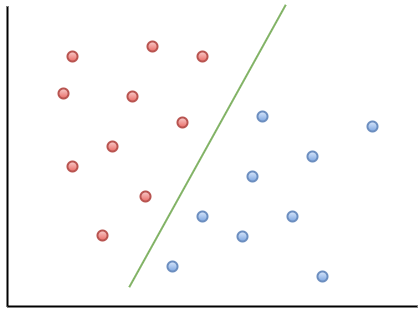
\includegraphics[height=4cm]{images/linsep.png}}
  \begin{itemize}
	\item Simplest way to separate data is a {\color{red} line} (or a {\color{red} hyperplane} in higher dimensions)
	\item Hypothesis class: linear combination of features
  \end{itemize}
\end{frame}

\section{Perceptron}

\begin{frame}
  \frametitle{Perceptron}
  \begin{itemize}
	\item Algorithm for {\color{red} binary classification}: $\mathcal{Y}=\{-1,+1\}$
	\item Assume inputs $x=(x_1,\ldots,x_d)$ on $d$ {\color{green} numerical} features
	\item Compute a {\color{blue} weighted score} and output $+1$ if
	\[\sum_{i=1}^d w_ix_i>\theta,\]
	otherwise output $\;-1$
  \end{itemize}
\end{frame}

\begin{frame}
  \frametitle{Perceptron}
  \begin{itemize}
	\item Sign function $\mathrm{sign}(x)$ outputs $+1$ if $x>0$ and $-1$ otherwise
	\item Hypothesis $h$ completely defined by {\color{green} weights} $w_0,\ldots,w_d$:
	\[h(x)=\mathrm{sign}\left(\sum_{i=1}^d w_ix_i-\theta\right)=\mathrm{sign}\left(\sum_{{\color{red} i=0}}^d w_ix_i\right)=\mathrm{sign}\left(w^\top x\right)\]
	where $x_0=1$ is a {\color{red} dummy feature} and $w_0=-\theta$
	\pause
	\item $\mathcal{H}$ is {\color{blue} infinite} (weights are real-valued)
	\item Classification loss: $\ell(h(x_i),y_i)=[h(x_i) \neq y_i]$
	\item $L_S(h) = \frac 1 m \sum_{i=1}^m [h(x_i) \neq y_i]$
  \end{itemize}
\end{frame}

\begin{frame}
  \frametitle{Linearly separable data}
  \begin{center}
  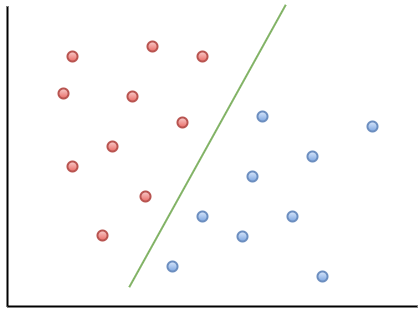
\includegraphics[height=5cm]{images/linsep.png}
  \end{center}
\end{frame}

\begin{frame}
  \frametitle{Perceptron learning algorithm (PLA)}
  \begin{block}{Perceptron learning algorithm}
  \begin{enumerate}
	\item Initialize weight vector $w_0=0$
	\item Find a {\color{red} mistake} $(x_i,y_i)$ such that $h(x_i)=\mathrm{sign}(w_0^\top x_i) \neq y_i$
	\item Update weights as $w_1\leftarrow w_0+y_ix_i$
	\item Repeat from 2. for weight vector $w_t$, $t=1,2,\ldots$
  \end{enumerate}
  \end{block}
\end{frame}

\begin{frame}
  \frametitle{Properties}
  \begin{itemize}
	\item If data is {\color{red} linearly separable}, PLA guaranteed to converge to a hypothesis $h_S$ (i.e.~weight vector $w_S$) such that $L_S(h_S)=0$
	\item If data is {\color{blue} not} linearly separable, PLA never converges
	\item Variants:
  \begin{itemize}
	\item Fix number of iterations $T$, stop when $t>T$
	\item {\color{green} Pocket algorithm}: only update weight vector $w_t$ when total number of mistakes decreases
  \end{itemize}
  \end{itemize}
\end{frame}

\section{Linear regression}

\begin{frame}
  \frametitle{Linear regression}
  \begin{itemize}
	\item Assumes {\color{red} regression problem} ($\mathcal{Y}=\mathbb{R}$)
	\item Hypothesis $h(x)=\sum_{i=0}^d w_ix_i=w^\top x$
	\item Squared loss: $\ell(h(x_i),y_i) = (h(x_i)-y_i)^2$
	\item $L_S(h) = \frac 1 m \sum_{i=1}^m (h(x_i)-y_i)^2$ is the {\color{green} mean squared error} (MSE)
  \end{itemize}
  \begin{center}
  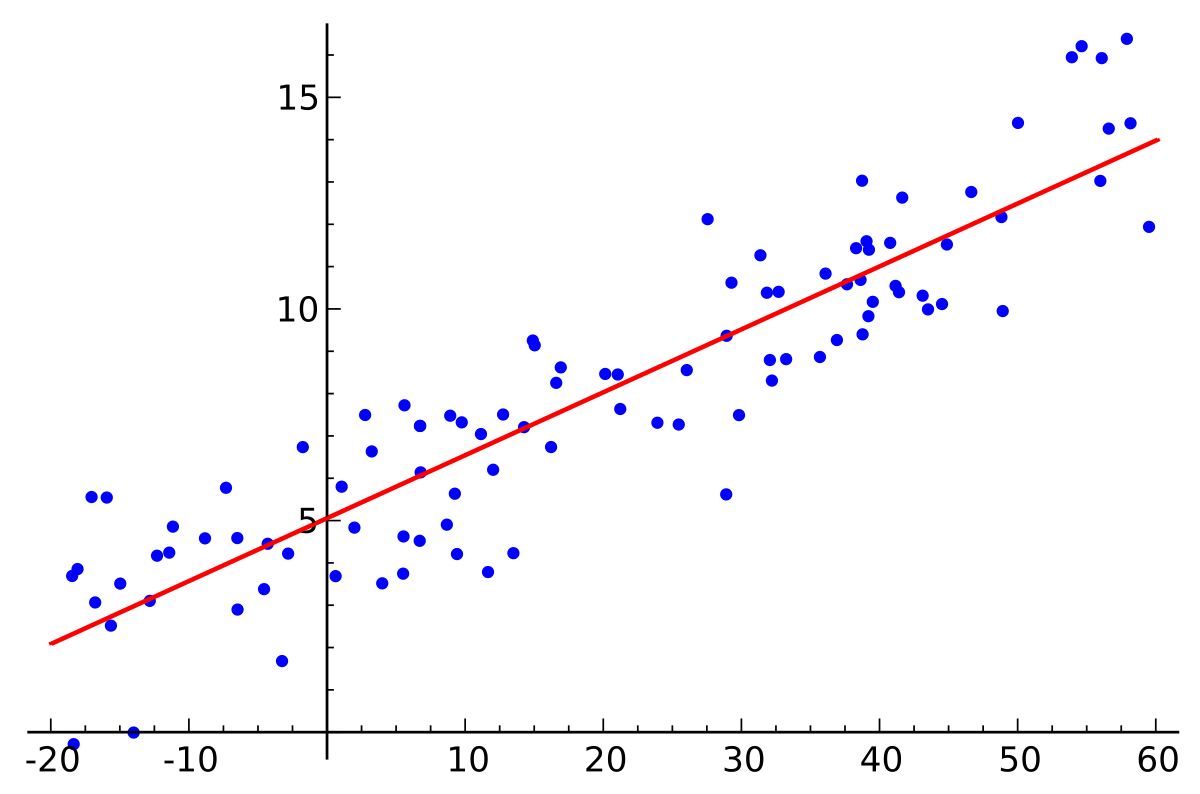
\includegraphics[height=3cm]{images/linreg.png}
  \end{center}
\end{frame}

\begin{frame}
  \frametitle{Linear regression}
  \begin{itemize}
	\item Hypothesis $h$ defined by {\color{green} weight vector} $w=(w_0,\ldots,w_d)$
	\item Find $w$ that minimizes
	\[L_S(w)=\frac 1 m \sum_{i=1}^m(h(x_i)-y_i)^2=\frac 1 m \sum_{i=1}^m(w^\top x_i-y_i)^2\]
	\item $L_S(w)$ is {\color{red} continuous}, {\color{red} differentiable}, and {\color{red} convex}
  \end{itemize}
\end{frame}

\begin{frame}
  \frametitle{Linear regression}
  \[
  \begin{cases}
  \begin{aligned}
  \action<+->{ L_S(w) &= \frac 1 m \sum_{i=1}^m(w^\top x_i-y_i)^2 = \frac 1 m \left \lVert \left( \begin{array}{c} w^\top x_1 - y_1\\ \vdots \\ w^\top x_m - y_m \end{array} \right) \right \rVert^2 \\}
  \action<+->{  &= \frac 1 m \left \lVert \left( \begin{array}{ccc} \textrm{-----} & x_1 & \textrm{-----} \\ \textrm{-----} & x_2 & \textrm{-----} \\ & \vdots & \\ \textrm{-----} & x_m & \textrm{-----} \end{array} \right)
  \left( \begin{array}{c} w_0 \\ \vdots \\ w_d \end{array} \right) -
  \left( \begin{array}{c} y_1 \\ y_2 \\ \vdots \\ y_m \end{array} \right) \right \rVert^2 \\}
  \action<+->{  &= \frac 1 m \left \lVert X w - y \right \rVert^2 = \frac 1 m \left( w^\top X^\top X w - 2 w^\top X^\top y + y^\top y \right) }
  \end{aligned}
  \end{cases}
  \]
  \pause
  \begin{itemize}
	\item $X$: $m\times(d+1)$ matrix of inputs
	\item $y$: $m\times 1$ vector of labels
  \end{itemize}
\end{frame}

\begin{frame}
  \frametitle{Linear regression}
  \begin{itemize}
	\item Minimize $L_S(w) \;\; \Leftrightarrow \;\;$ set {\color{red} gradient} $\nabla_w L_S(w)$ to $0$
	\[
	\nabla_w L_S(w) = \left( \begin{array}{c} \frac {\partial L_S(w)} {\partial w_0} \\ \vdots \\ \frac {\partial L_S(w)} {\partial w_d} \end{array} \right)
	\]
	\pause
	\item Single term $(w^\top x_1 - y_1)^2$, single weight $w_0$:
  \[
	\frac {\partial (w^\top x_1 - y_1)^2} {\partial w_0} = 2(w^\top x_1 - y_1) x_{10}
  \]
	\pause
	\item {\color{red} Gradient}
	\[\nabla_w L_S(w)=\frac{2}{m}(X^\top X w - X^\top y)\]
  \end{itemize}
\end{frame}

\begin{frame}
  \frametitle{Linear regression}
  \begin{itemize}
	\item $\nabla_w L_S(w) = 0 \;\; \Leftrightarrow \;\; X^\top X w = X^\top y$
	\item $X^\top X$ is a $(d+1)\times(d+1)$ matrix
	\pause
	\vspace*{0.5cm}
	\item $X^\top X$ invertible: {\color{blue} Analytic solution} $w_{\mathrm{lin}} = (X^\top X)^{-1}X^\top y = X^\dagger y$
	\item $X^\dagger = (X^\top X)^{-1}X^\top$: {\color{green} pseudo-inverse} of $X$
	\item {\color{cyan} In practice}: use well-implemented $\dagger$ routine for computing $X^\dagger$
  \end{itemize}
\end{frame}

\begin{frame}
  \frametitle{Hat matrix}
  \begin{center}
  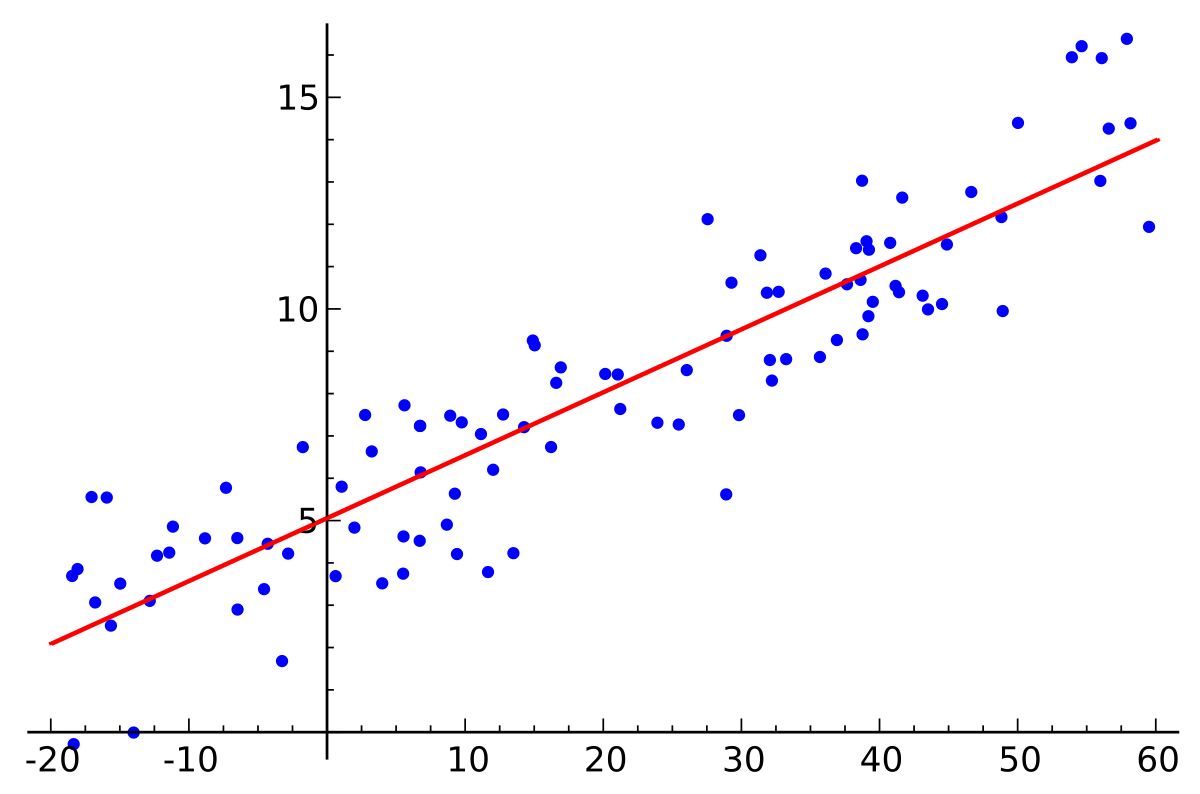
\includegraphics[height=3cm]{images/linreg.png}
  \end{center}
  \begin{itemize}
	\item Approximate labels on inputs $x_1,\ldots,x_m$:
	\[
	\hat{y} = X w_{\mathrm{lin}} = X(X^\top X)^{-1}X^\top y = H y
	\]
	\item $H=X(X^\top X)^{-1}X^\top$ is called the {\color{red} hat matrix} since it puts the ``hat'' on $y$
  \end{itemize}
\end{frame}

\begin{frame}
  \frametitle{Is linear regression really ``learning''?}
  \begin{itemize}
	\item {\color{red} No}, in the sense that $w_{\mathrm{lin}}$ has an {\color{red} analytical solution}
	\item No algorithm necessary for iteratively improving the training loss
	\item {\color{green} Yes}, in the sense that we achieve a small training loss $L_S(w)$
	\item Algorithm for computing the pseudo-inverse $X^\dagger = (X^\top X)^{-1}X^\top$
  \end{itemize}
\end{frame}

\begin{frame}
  \frametitle{Linear classification vs.~linear regression}
  \begin{itemize}
	\item Minimizing $L_S(h) = \frac 1 m \sum_{i=1}^m [h(x_i) \neq y_i]$ is {\color{red} NP-hard}
	\item Minimizing $L_S(h) = \frac 1 m \sum_{i=1}^m (h(x_i) - y_i)^2$ has an {\color{green} efficient analytical solution}
	\item {\color{blue} Idea}: $\{-1,+1\} \subset \mathbb{R}$ $\Rightarrow$ use linear regression for classification!
	\item On input $x$, predict label $\mathrm{sign}(w_{\mathrm{lin}}^\top x)$
  \end{itemize}
\end{frame}

\begin{frame}
  \frametitle{Relationship between loss functions}
  \begin{center}
  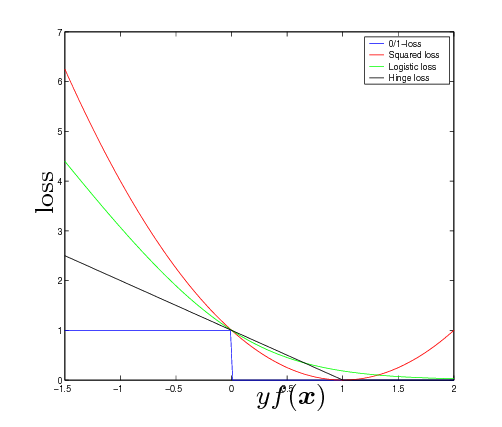
\includegraphics[height=5cm]{images/losses.png}
  \end{center}
  \begin{itemize}
	\item For label $+1$, square loss upper bounds 0-1 loss! (same for $-1$)
	\item Sacrifice {\color{red} bound tightness} for {\color{green} efficiency}
  \end{itemize}
\end{frame}

\section{Logistic regression}

\begin{frame}
  \frametitle{Logistic regression}
  \begin{itemize}
	\item {\color{red} Soft classification}: estimate {\color{blue} probability} of belonging to class
	\item Hypothesis $h(x)=\theta(\sum_{i=0}^d w_ix_i)=\theta(w^\top x)$
	\item {\color{green} Logistic function}
	\[\theta(s)=\frac{1}{1+e^{-s}}\]
  \end{itemize}
  \begin{center}
  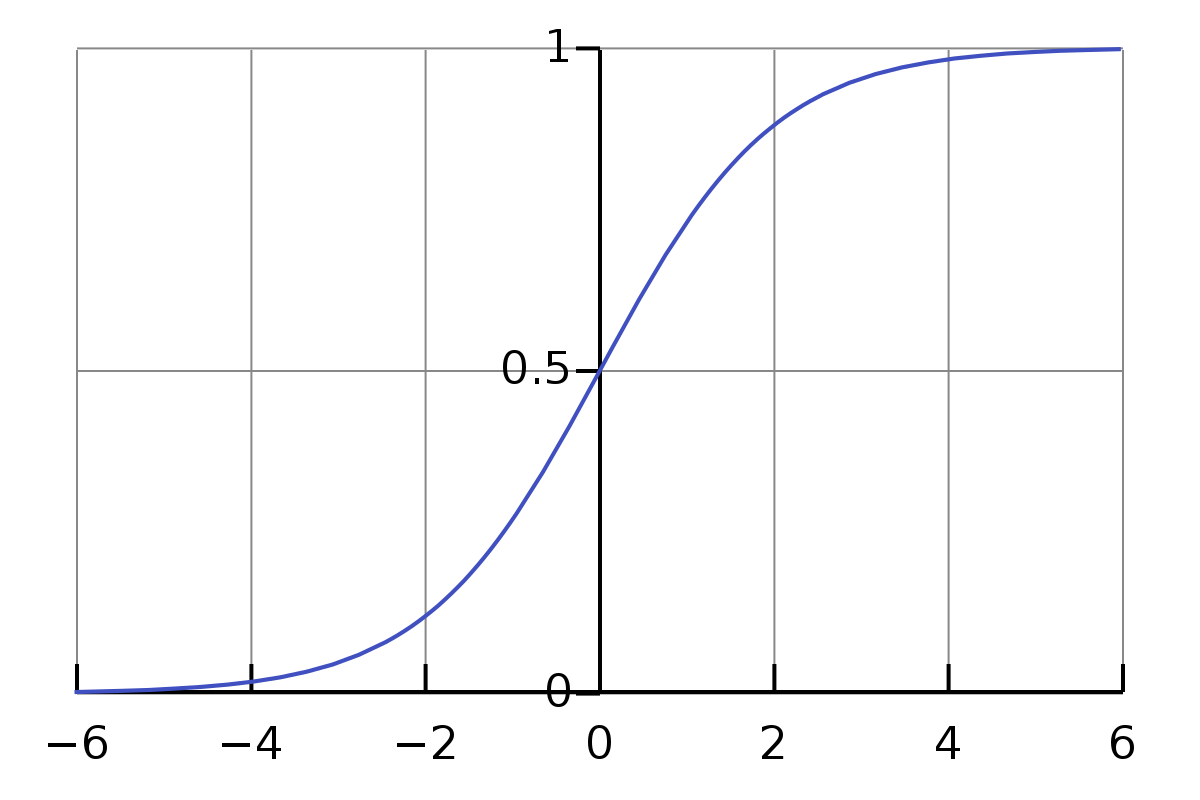
\includegraphics[height=3cm]{images/sigmoid.png}
  \end{center}
\end{frame}

\begin{frame}
  \frametitle{Logistic regression}
  \begin{itemize}
	\item Assume that there are two classes $\{-1,+1\}$
	\item Ideally, data would be on the form $((x_1,0.8),\ldots,(x_m,0.1))$, i.e.~the {\color{red} probability} of belonging to class $+1$
	\item However, data is usually on the form $((x_1,+1),\ldots,(x_m,-1))$
	\item We can view labels as {\color{blue} hard probabilities}, i.e.~$0$ or $1$
  \end{itemize}

  \vspace*{1cm}

  \begin{center}
  \begin{tikzpicture}[overlay]
	\node at (0,0) {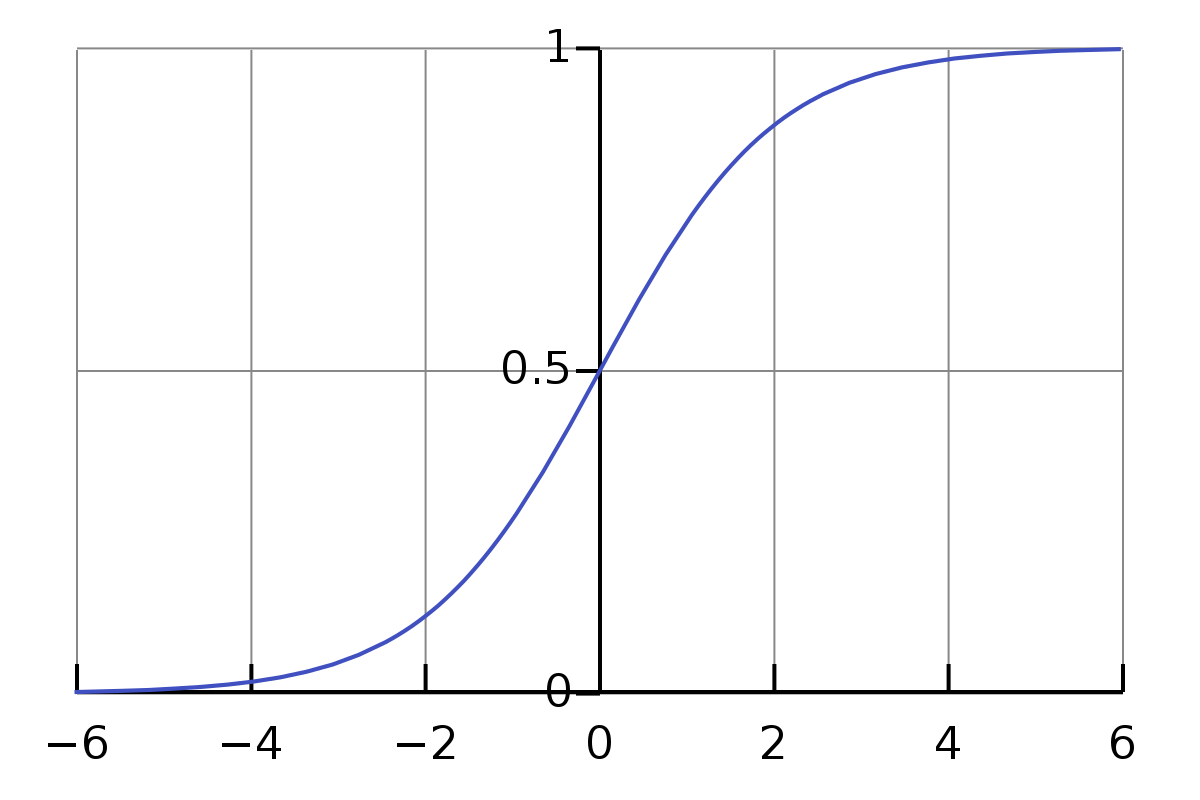
\includegraphics[height=3cm]{images/sigmoid.png}};
	\draw[color=red,thick=2pt] (-1.6,-1.05) -- (-1.5,-1.15);
	\draw[color=red,thick=2pt] (-1.6,-1.15) -- (-1.5,-1.05);
	\draw[color=red,thick=2pt] (-1.3,-1.05) -- (-1.2,-1.15);
	\draw[color=red,thick=2pt] (-1.3,-1.15) -- (-1.2,-1.05);
	\draw[color=red,thick=2pt] (-0.7, 1.25) -- (-0.6, 1.35);
	\draw[color=red,thick=2pt] (-0.7, 1.35) -- (-0.6, 1.25);
	\draw[color=red,thick=2pt] (-0.4,-1.05) -- (-0.3,-1.15);
	\draw[color=red,thick=2pt] (-0.4,-1.15) -- (-0.3,-1.05);
	\draw[color=red,thick=2pt] ( 0.3, 1.25) -- ( 0.4, 1.35);
	\draw[color=red,thick=2pt] ( 0.3, 1.35) -- ( 0.4, 1.25);
	\draw[color=red,thick=2pt] ( 0.6,-1.05) -- ( 0.7,-1.15);
	\draw[color=red,thick=2pt] ( 0.6,-1.15) -- ( 0.7,-1.05);
	\draw[color=red,thick=2pt] ( 1.3, 1.25) -- ( 1.2, 1.35);
	\draw[color=red,thick=2pt] ( 1.3, 1.35) -- ( 1.2, 1.25);
	\draw[color=red,thick=2pt] ( 1.6, 1.25) -- ( 1.7, 1.35);
	\draw[color=red,thick=2pt] ( 1.6, 1.35) -- ( 1.7, 1.25);
  \end{tikzpicture}
  \end{center}
\end{frame}

\begin{frame}
  \frametitle{Logistic loss}
  \begin{itemize}
	\item Find $w$ that minimizes
	\[L_S(w) = \frac 1 m \sum_{i=1}^m \ell(h(x_i),y_i)\]
	\item {\color{blue} Cross-entropy loss} $\ell(h(x_i),y_i)=\ln(1+\mathrm{exp}(-y_i w^\top x_i))$
	\item $L_S(w)$ is {\color{red} continuous}, {\color{red} differentiable}, and {\color{red} convex}
  \end{itemize}
\end{frame}

\begin{frame}
  \frametitle{Logistic loss}
  \begin{itemize}
	\item Minimize $L_S(w) \;\; \Leftrightarrow \;\;$ Find $w$ such that $\nabla_w L_S(w) = 0$
	\item {\color{blue} Gradient}
	\[\nabla_w L_S(w) = \frac 1 m \sum_{i=1}^m \theta(-y_i w^\top x_i)(-y_ix_i)\]
	\item Unfortunately, no analytic solution to $\nabla_w L_S(w) = 0$
	\pause
	\item (Stay tuned for {\color{red} optimization and gradient descent})
  \end{itemize}
\end{frame}

\begin{frame}
  \frametitle{Multiclass classification}
  \begin{itemize}
	\item So far we have mainly talked about binary classification, i.e.~$|\mathcal{Y}|=2$
	\item What if there are more than two classes, i.e.~$2<|\mathcal{Y}|=k$?
	\item Two main approaches:
	\begin{enumerate}
	\item {\color{red} One-versus-all (OVA)}: {\color{blue} binary} classification of one class vs. rest
	\item {\color{red} One-versus-one (OVO)}: {\color{blue} binary} classification of pairs of classes
	\end{enumerate}
	\item In both cases, perform soft binary classification (i.e.~logistic regression) and return {\color{green} most probable class}
  \end{itemize}
\end{frame}

\begin{frame}
  \frametitle{One-versus-all}
  \begin{center}
  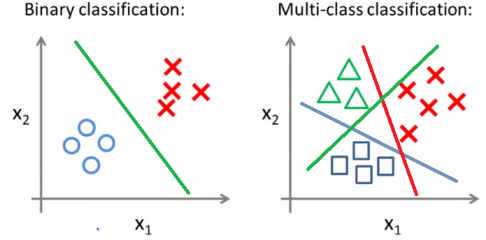
\includegraphics[height=4cm]{images/multiclass.png}
  \end{center}
\end{frame}

\begin{frame}
  \frametitle{Multiclass classification}
  Properties of one-versus-all (OVA):
  \begin{itemize}
	\item Linear number of classifiers
	\item Imbalanced data!
  \end{itemize}
  Properties of one-versus-one (OVO):
  \begin{itemize}
	\item Quadratic number of classifiers
	\item More balanced data
  \end{itemize}
\end{frame}

\section{Non-linear transforms}

\begin{frame}
  \frametitle{Non-linear data}
  \begin{center}
  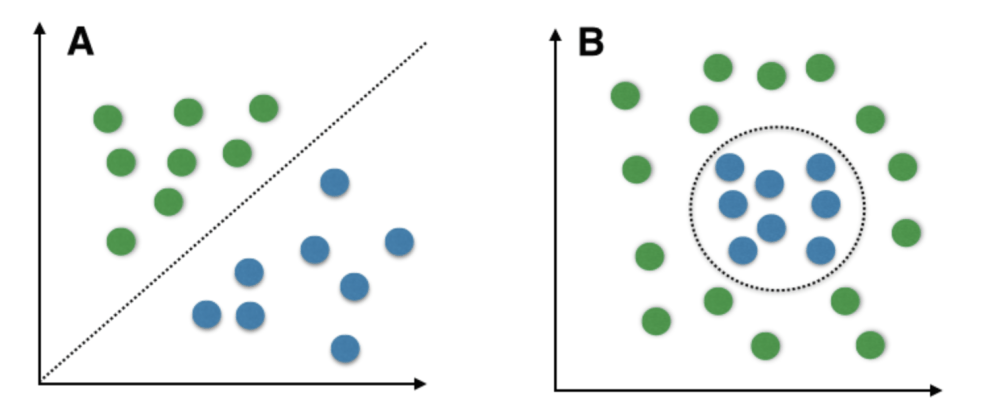
\includegraphics[height=3cm]{images/circular.png}
  \end{center}
  \begin{itemize}
	\item Often data is not linearly separable at all
	\item {\color{red} Idea}: derive {\color{blue} circular} perceptron, {\color{blue} circular} regression, etc.
	\item It would be better to take advantage of linear models!
  \end{itemize}
\end{frame}

\begin{frame}
  \frametitle{Non-linear transforms}
  \begin{center}
  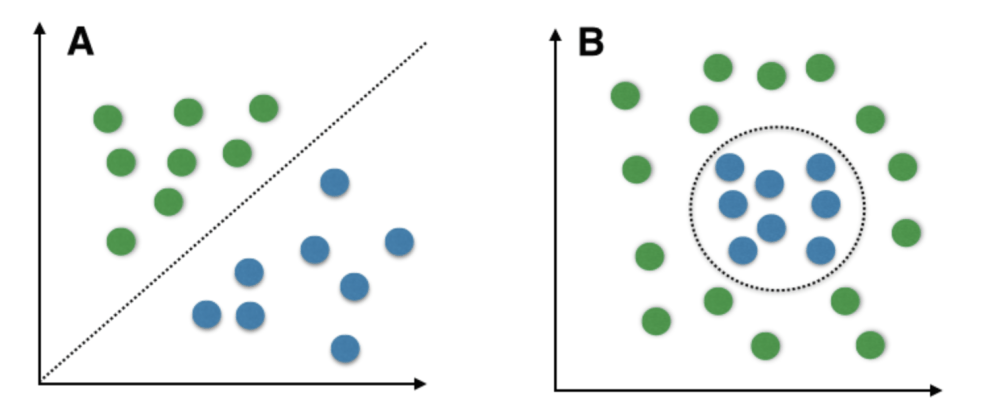
\includegraphics[height=3cm]{images/circular.png}
  \end{center}
  \begin{itemize}
	\item Circular hypothesis: $h(x)=\mathrm{sign}(0.6-x_1^2-x_2^2)$
	\item Linear in {\color{red} quadratic terms} $x_1^2$ and $x_2^2$!
	\item Non-linear transform: introduce additional {\color{blue} non-linear terms}
	\item Quadratic transform: $z=\Phi(x)=(1,x_1,x_2,x_1x_2,x_1^2,x_2^2)$
  \end{itemize}
\end{frame}

\begin{frame}
  \frametitle{Non-linear transforms}
  \begin{center}
  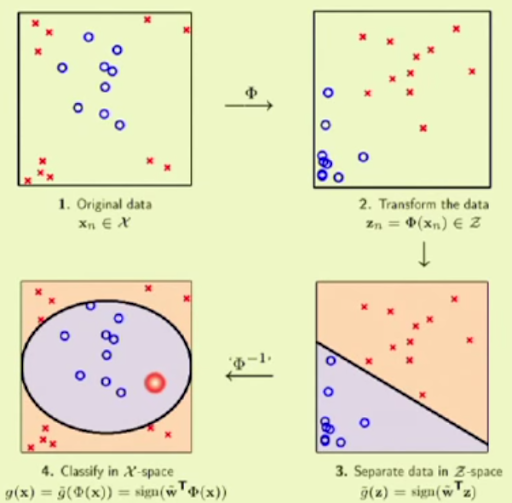
\includegraphics[height=5cm]{images/nonlin.png}
  \end{center}
  \begin{itemize}
	\item Transform each data point $(x_i,y_i)$ to $(z_i=\Phi(x_i),y_i)$
	\item Apply linear algorithm in transformed space to find $\tilde{w}$
	\item Hypothesis on input $x$ proportional to $\tilde{w}^\top \Phi(x)$
  \end{itemize}
\end{frame}

\begin{frame}
  \frametitle{Price of non-linear transforms}
  \begin{itemize}
	\item Let $\mathcal{H}_q$ be the hypothesis class of $q$-th order polynomials
	\item Then $\mathcal{H}_1 \subset \mathcal{H}_2 \subset \cdots \subset \mathcal{H}_q$
	\item However, number of features increases!
	\item The $q$-th order polynomial has $O(d^q)$ dimensions
	\item Increases memory requirements, running time of algorithms, etc.
  \end{itemize}
\end{frame}

\section{Exercises}

\begin{frame}
  \frametitle{Multiclass classification}
  \begin{itemize}
  \item Assume that a binary classification algorithm $\mathcal{A}$ runs in time $N^3$ on data of size $N$
  \item For a 10 class classification problem ($|\mathcal{Y}|=10$), assume that there are exactly $N/10$ data points for each class
  \item What is the running time of OVA and OVO multiclass classification using algorithm $\mathcal{A}$?
  \end{itemize}
\end{frame}

\begin{frame}
  \frametitle{One-versus-all (OVA)}
  \begin{itemize}
  \item We have to build 10 classifiers in total
  \pause
  \item Each classifier uses {\color{red} all data}, i.e.~$N$ data points
  \pause
  \item For each classifier, the running time of algorithm $\mathcal{A}$ is $N^3$
  \pause
  \item Hence the total running time is $10N^3$
  \end{itemize}
\end{frame}

\begin{frame}
  \frametitle{One-versus-one (OVO)}
  \begin{itemize}
  \item We have to build $\left( \begin{array}{c} 10\\ 2 \end{array} \right)=\frac {10\cdot 9} 2 = 45$ classifiers in total
  \pause
  \item Each classifier uses only data points of 2 classes, i.e.~$2N/10$
  \pause
  \item For each classifier, the running time of algorithm $\mathcal{A}$ is $8N^3/1000$
  \pause
  \item Hence the total running time is $45\cdot 8N^3/1000 = \frac 9 {25} N^3$
  \end{itemize}
\end{frame}

\begin{frame}
  \frametitle{Non-linear transforms}
  \begin{itemize}
  \item Consider the hypothesis class $\mathcal{H}_2$ of second-order polynomials
  \item Let $d$ be the number of dimensions of the original inputs $x\in\mathcal{X}$
  \item What is the number of dimensions of transformed inputs $z=\Phi(x)$?
  \item Recall that the features are $1,x_1,\ldots,x_d,x_1^2,x_1x_2,x_2^2,\ldots$
  \end{itemize}
\end{frame}

\begin{frame}
  \frametitle{Non-linear transforms}
  \begin{itemize}
  \item $\mathcal{H}_2$ contains {\color{red} quadratic}, {\color{red} linear} and {\color{red} constant} terms
  \pause
  \item The number of quadratic terms is $\left( \begin{array}{c} d\\ 2 \end{array} \right) + d = \frac {d(d-1)+2d} 2 = \frac{d^2 + d} 2$
  \pause
  \item The number of linear terms is $d$
  \pause
  \item The number of constant terms is $1$ (the dummy feature $+1$)
  \pause
  \item In total, there are $\frac{d^2 + d} 2 + d + 1 = {\color{green} \frac {d^2} 2 + \frac {3d} 2 + 1}$ terms
  \end{itemize}
\end{frame}

\begin{frame}
  \frametitle{Linear regression}
	The training loss for linear regression is given by
  \begin{align}
	L_S(w)=\frac 1 m (w^\top X^\top X w - 2 w^\top X^\top y + y^\top y).
  \end{align}
	Assuming that $X^\top X$ is invertible, show that $L_S(w)$ can be written as
  \begin{align}
	L_S(w) = \frac 1 m (&(w - w_{\mathrm{lin}})^\top (X^\top X)(w - w_{\mathrm{lin}}) + y^\top (y - Xw_{\mathrm{lin}}),
  \end{align}
	where $w_{\mathrm{lin}} = (X^\top X)^{-1}X^\top y$ is the weight vector that minimizes empirical risk
\end{frame}

\begin{frame}
  \frametitle{Linear regression}
  Multiplying $X^\top X$ with $w_{\mathrm{lin}}$ yields
  \begin{align*}
	(X^\top X)w_{\mathrm{lin}} &= (X^\top X)(X^\top X)^{-1}X^\top y = I\,X^\top y = X^\top y.
  \end{align*}
  Using the properties of the transpose yields
  \begin{align*}
	w_{\mathrm{lin}}^\top(X^\top X) &= ((X^\top X)w_{\mathrm{lin}})^\top = (X^\top y)^\top = y^\top X.
  \end{align*}
\end{frame}

\begin{frame}
  \frametitle{Linear regression}
  Show that simplifying (2) results in (1):
  \[
  \begin{cases}
  \begin{aligned}
  \action<+->{m & L_S(w) = (w - w_{\mathrm{lin}})^\top (X^\top X)(w - w_{\mathrm{lin}}) + y^\top (y - Xw_{\mathrm{lin}}) \\}
  \action<+->{ &= (w - w_{\mathrm{lin}})^\top (X^\top Xw - {\color{red} X^\top X w_{\mathrm{lin}}} ) + y^\top (y - Xw_{\mathrm{lin}}) \\}
  \action<+->{ &= (w - w_{\mathrm{lin}})^\top (X^\top Xw - X^\top y) + y^\top (y - Xw_{\mathrm{lin}}) \\}
  \action<+->{ &= w^\top X^\top Xw - {\color{red} w_{\mathrm{lin}}^\top X^\top X} w - w^\top  X^\top y + w_{\mathrm{lin}}^\top X^\top y + y^\top y - y^\top Xw_{\mathrm{lin}} \\}
  \action<+->{ &= w^\top X^\top Xw - y^\top X w - w^\top X^\top y + w_{\mathrm{lin}}^\top X^\top y + y^\top y - y^\top Xw_{\mathrm{lin}} \\}
  \action<+->{ &= \{ y^\top X w \; \text{and} \; y^\top Xw_{\mathrm{lin}} \; \text{are} \; \text{\color{red} scalars} \; \Leftrightarrow y^\top X w = w^\top X^\top y \} \\}
  \action<+->{ &= w^\top X^\top Xw - w^\top X^\top y - w^\top X^\top y + \hcancel[red]{w_{\mathrm{lin}}^\top X^\top y} + y^\top y - \hcancel[red]{w_{\mathrm{lin}}^\top X^\top y} \\}
  \action<+->{ &= w^\top X^\top Xw - 2 w^\top X^\top y + y^\top y }
  \end{aligned}
  \end{cases}
  \]
\end{frame}

\begin{frame}
  \frametitle{Linear regression}
	The matrix $X^\top X$ is positive definite, i.e.~for any vector $v$,
	\[
	v^\top (X^\top X) v \geq 0.
	\]
	Trivially, the expression
  \begin{align*}
	L_S(w) = \frac 1 m (&(w - w_{\mathrm{lin}})^\top (X^\top X)(w - w_{\mathrm{lin}}) + y^\top (y - Xw_{\mathrm{lin}})
  \end{align*}
	is minimized when $w - w_{\mathrm{lin}} = 0$, i.e.~when $w = w_{\mathrm{lin}}$
\end{frame}

\begin{comment}
\begin{frame}
  \frametitle{Hat matrix}
  Show that the hat matrix $H=X(X^\top X)^{-1}X^\top$ has the following properties (where $I$ is the {\color{red} identity matrix}):
  \begin{enumerate}
  \item $H$ is symmetric, i.e.~$H^\top = H$
  \item $H^2 = H$
  \item $(I-H)^2 = (I-H)$
  \end{enumerate}
\end{frame}

\begin{frame}
  \frametitle{Hat matrix}
  Note that $(AB)^\top = B^\top A^\top$ and that $\left(A^{-1}\right)^\top = \left(A^\top\right)^{-1}$
  \[
  \begin{cases}
  \begin{aligned}
  \action<+->{H^\top &= \left( X(X^\top X)^{-1}X^\top \right)^\top \\}
  \action<+->{ &= X \left( (X^\top X )^{-1} \right)^\top X^\top \\}
  \action<+->{ &= X \left( (X^\top X )^\top \right)^{-1} X^\top \\}
  \action<+->{ &= X \left( X^\top X \right)^{-1} X^\top = H }
  \end{aligned}
  \end{cases}
  \]
\end{frame}

\begin{frame}
  \frametitle{Hat matrix}
  Note that $A^{-1} A = I$ and $AI = IA = A$
  \[
  \begin{cases}
  \begin{aligned}
  \action<+->{H^2 &= H \cdot H = X(X^\top X)^{-1}X^\top X(X^\top X)^{-1}X^\top \\}
  \action<+->{ &= X {\color{red} (X^\top X)^{-1} (X^\top X)} (X^\top X)^{-1}X^\top \\}
  \action<+->{ &= X {\color{red} I} (X^\top X)^{-1}X^\top \\}
  \action<+->{ &= X (X^\top X)^{-1}X^\top = H }
  \end{aligned}
  \end{cases}
  \]
\end{frame}

\begin{frame}
  \frametitle{Hat matrix}
  \[
  \begin{cases}
  \begin{aligned}
  \action<+->{(I-H)^2 &= I^2 - 2IH + H^2 \\}
  \action<+->{ &= I - 2H + H = I - H}
  \end{aligned}
  \end{cases}
  \]
\end{frame}
\end{comment}

\begin{comment}
\begin{frame}
  \frametitle{Perceptron learning algorithm (PLA)}
  If $(x_i,y_i)$ is a mistake, $\mathrm{sign}(w_t^\top x_i) \neq y_i \Leftrightarrow {\color{red} y_iw_t^\top x_i \leq 0}$
  \begin{block}{Perceptron learning algorithm}
  \begin{enumerate}
	\item Initialize weight vector $w_0=0$
	\item Find a {\color{red} mistake} $(x_i,y_i)$ such that $h(x_i)\neq y_i$
	\item Update weights as $w_1\leftarrow w_0+y_ix_i$
	\item Repeat from 2. for weight vector $w_t$, $t=1,2,\ldots$
  \end{enumerate}
  \end{block}
  Show that after iteration $t$ it holds that {\color{red} $y_iw_{t+1}^\top x_i > y_iw_t^\top x_i$}\\
  Hence PLA attempts to {\color{green} correct} the mistake on $(x_i,y_i)$
\end{frame}

\begin{frame}
  \frametitle{Perceptron learning algorithm (PLA)}
  
  \[
  \begin{cases}
  \begin{aligned}
  \action<+->{y_iw_{t+1}^\top x_i &= y_i \left( w_t + y_ix_i \right)^\top x_i \\}
  \action<+->{&= y_iw_t^\top x_i + {\color{red} y_i^2} x_i^\top x_i \\}
  \action<+->{&= y_iw_t^\top x_i + x_i^\top x_i \\}
  \action<+->{&= y_iw_t^\top x_i + \lVert x_i \rVert^2 \\}
  \action<+->{&\geq y_iw_t^\top x_i + {\color{red} 1} > y_iw_t^\top x_i}
  \end{aligned}
  \end{cases}
  \]
\end{frame}
\end{comment}

\begin{frame}
  \frametitle{Perceptron learning algorithm (PLA)}
  \begin{block}{Perceptron learning algorithm}
  \begin{enumerate}
	\item Initialize weight vector $w_0=0$
	\item Find a {\color{red} mistake} $(x_i,y_i)$ such that $h(x_i)\neq y_i$
	\item Update weights as $w_1\leftarrow w_0+y_ix_i$
	\item Repeat from 2. for weight vector $w_t$, $t=1,2,\ldots$
  \end{enumerate}
  \end{block}
  Letting $R^2=\max_i \lVert x_i \rVert^2$, show that after $t$ iterations, $\lVert w_t \rVert^2 \leq t R^2$ 
\end{frame}

\begin{frame}
  \frametitle{Perceptron learning algorithm (PLA)}
  
  Consider a single step of PLA:
  \[
  \begin{cases}
  \begin{aligned}
  \action<+->{\lVert w_{t+1} \rVert^2 &= \lVert w_t + y_ix_i \rVert^2 \\}
  \action<+->{&= \lVert w_t \rVert^2 + 2 y_iw_t^\top x_i + {\color{red} y_i^2} \lVert x_i \rVert^2 \\}
  \action<+->{&\leq \lVert w_t \rVert^2 + {\color{red} 0} + \lVert x_i \rVert^2 \\}
  \action<+->{&\leq \lVert w_t \rVert^2 + R^2}
  \end{aligned}
  \end{cases}
  \]
  \pause
  Hence after $t$ iterations, $\lVert w_t \rVert^2 \leq \lVert w_0 \rVert^2 + tR^2 = 0 + tR^2 = tR^2$
\end{frame}

\begin{frame}
  \frametitle{Perceptron learning algorithm (PLA)}
  Data linearly separable $\Rightarrow$ exists $w_*$ such that $y_iw_*^\top x_i > 0, \; \forall i\in[m]$
  \begin{block}{Perceptron learning algorithm}
  \begin{enumerate}
	\item Initialize weight vector $w_0=0$
	\item Find a {\color{red} mistake} $(x_i,y_i)$ such that $h(x_i)\neq y_i$
	\item Update weights as $w_1\leftarrow w_0+y_ix_i$
	\item Repeat from 2. for weight vector $w_t$, $t=1,2,\ldots$
  \end{enumerate}
  \end{block}
  Letting $\rho = \min_i y_i \frac {w_*^\top} {\lVert w_* \rVert} x_i>0$,
  show that after $t$ iterations, $\frac {w_*^\top w_t} {\lVert w_* \rVert} \geq t \rho$
\end{frame}

\begin{frame}
  \frametitle{Perceptron learning algorithm (PLA)}
  
  Consider a single step of PLA:
  \[
  \begin{cases}
  \begin{aligned}
  \action<+->{\frac {w_*^\top w_{t+1}} {\lVert w_* \rVert} &= \frac {w_*^\top w_t} {\lVert w_* \rVert} + y_i \frac {w_*^\top} {\lVert w_* \rVert} x_i \\}
  \action<+->{&\geq \frac {w_*^\top w_t} {\lVert w_* \rVert} + \rho}
  \end{aligned}
  \end{cases}
  \]
  \pause
  Hence after $t$ iterations, $\frac {w_*^\top w_t} {\lVert w_* \rVert} \geq \frac {w_*^\top w_0} {\lVert w_* \rVert} + t\rho = 0 + t\rho = t\rho$
\end{frame}

\begin{frame}
  \frametitle{Perceptron learning algorithm (PLA)}
  \begin{itemize}
  \item Putting the two results together, we get
  \[
  \frac {w_*^\top w_t} {\lVert w_* \rVert \lVert w_t \rVert} \geq \frac {t\rho} {\sqrt{t}R} = \sqrt{t} \frac \rho R
  \]
  \pause
  \item The scalar product of two unit vectors is upper bounded by $1$:
  \[
	1 \geq \frac {w_*^\top w_t} {\lVert w_* \rVert \lVert w_t \rVert} \geq \sqrt{t} \frac \rho R
  \]
  \pause
  \item It follows that
  \[
	\sqrt{t} \leq \frac R \rho \;\; \Leftrightarrow \;\; t \leq \frac {R^2} {\rho^2}
  \]
  \pause
  \item Hence PLA converges after at most $R^2/\rho^2$ iterations!
  \end{itemize}
\end{frame}

\end{document}

